\chapter{Anhang}
\section{Liste bestehender Rails 2 und 3 Web Content Management Systeme bzw. Blogging-Software}

\begin{table}[!ht]
\center
\begin{tabular}[]{|p{3cm}|p{8cm}|p{4cm}|}
% Begin Rails 2
\hline
\multicolumn{3}{|p{15cm}|}{\textbf{OpenSource Web Content Management Systeme mit Rails 2.x Unterstützung}}\\
\hline
\textbf{Projektname}&\textbf{Projektseite im Internet}&\textbf{Aktive Weiterentwicklung}\\
\hline
Alchemy CMS & \href{http://magiclabs.github.com/alchemy/}{http://magiclabs.github.com/alchemy/} & Ja \\
\hline
Skyline CMS & \href{http://www.skylinecms.nl/}{http://www.skylinecms.nl/} & Ja \\
\hline
Webiva & \href{http://webiva.org/}{http://webiva.org/} & Ja \\
\hline
Railfrog & \href{http://railfrog.com/}{http://railfrog.com/} & Nein \\
\hline
Radiant & \href{http://radiantcms.org/}{http://radiantcms.org/} & Ja \\
\hline
zenacms & \href{http://zenadmin.org/}{http://zenadmin.org/} & Ja \\
\hline
Compages & \href{http://compages.wordpress.com/}{http://compages.wordpress.com/} & eingestellt\\
\hline
Comatose & \href{http://comatose.rubyforge.org/}{http://comatose.rubyforge.org/} & eingestellt\\
\hline
Mephisto & \href{https://github.com/halorgium/mephisto}{https://github.com/halorgium/mephisto} & eingestellt\\
\hline
Rubricks & \href{http://rubricks.org/}{http://rubricks.org/} & eingestellt\\
\hline
Typhus & \href{http://typus.heroku.com/}{http://typus.heroku.com/} & eingestellt\\
\hline
Station & \href{https://github.com/atd/station}{https://github.com/atd/station} & Ja\\
\hline
Vrame & \href{https://github.com/9elements/vrame}{https://github.com/9elements/vrame} & eingestellt\\
\hline
Ansuz CMS & \href{https://github.com/knewter/ansuz}{https://github.com/knewter/ansuz} & eingestellt\\
\hline
Geego CMS & \href{http://gitorious.org/geego-cms\#more}{http://gitorious.org/geego-cms\#more} & eingestellt\\
\hline


\end{tabular}
\end{table}

% End Rails 2

% Begin Rails 3
\begin{table}
\center
\begin{tabular}[]{|p{3cm}|p{8cm}|p{4cm}|}
\hline
\multicolumn{3}{|p{15cm}|}{\textbf{Open Source Web Content Management Systeme mit Rails 3.x Unterstützung}}\\
\hline
\textbf{Projektname}&\textbf{Projektseite im Internet}&\textbf{Aktive Weiterentwicklung}\\
\hline
Alchemy CMS & \href{http://magiclabs.github.com/alchemy/}{http://magiclabs.github.com/alchemy/} & Ja \\
\hline
Browser CMS & \href{http://browsercms.org}{http://browsercms.org} & Ja \\
\hline
Locomotive CMS & \href{http://www.locomotivecms.com/}{http://www.locomotivecms.com/} & Ja \\
\hline
Refinery CMS & \href{http://refinerycms.com/}{http://refinerycms.com/} & Ja \\
\hline
adva-cms & \href{http://adva-cms.org/}{http://adva-cms.org/} & Ja \\
\hline
typo (Blogging) & \href{http://fdv.github.com/typo/}{http://fdv.github.com/typo/} & Ja \\
\hline
Surtout CMS & \href{http://surtoutcms.com/}{http://surtoutcms.com/} & noch nicht veröffentlicht \\
\hline
Nesta CMS\footnotemark[1] & \href{https://github.com/gma/nesta}{https://github.com/gma/nesta} & ja  \\
\hline
% End Rails 3
\end{tabular}
\footnotetext[1]{Nesta basiert auf dem Ruby Webframework Sinatra und kann in Rails 3 als Rack-Middleware integriert werden.}
\end{table}

% begin closed source
\begin{table}
\center
\begin{tabular}[]{|p{3cm}|p{8cm}|p{4cm}|}
\hline
\multicolumn{3}{|p{15cm}|}{\textbf{Closed Source Web Content Management Systeme mit Rails 3.x Unterstützung}}\\
\hline
\textbf{Projektname}&\textbf{Projektseite im Internet}&\textbf{Aktive Weiterentwicklung}\\
\hline
Blocks & \href{http://www.blocksglobal.com/}{http://www.blocksglobal.com/} & Ja \\
\hline
% End clsoed source
\end{tabular}
\end{table}


\newpage


\section{Crudify-Methode von Refinery CMS 1.0.8}


\lstinputlisting[label=crudify, nolol=true, title=Implementierung der Crudify-Methode in Refinery CMS 1.0.8,language=Ruby]{code/crudify_method.rb}

\section{Ext-Direct Spezifikation für Ext Js 3.0}

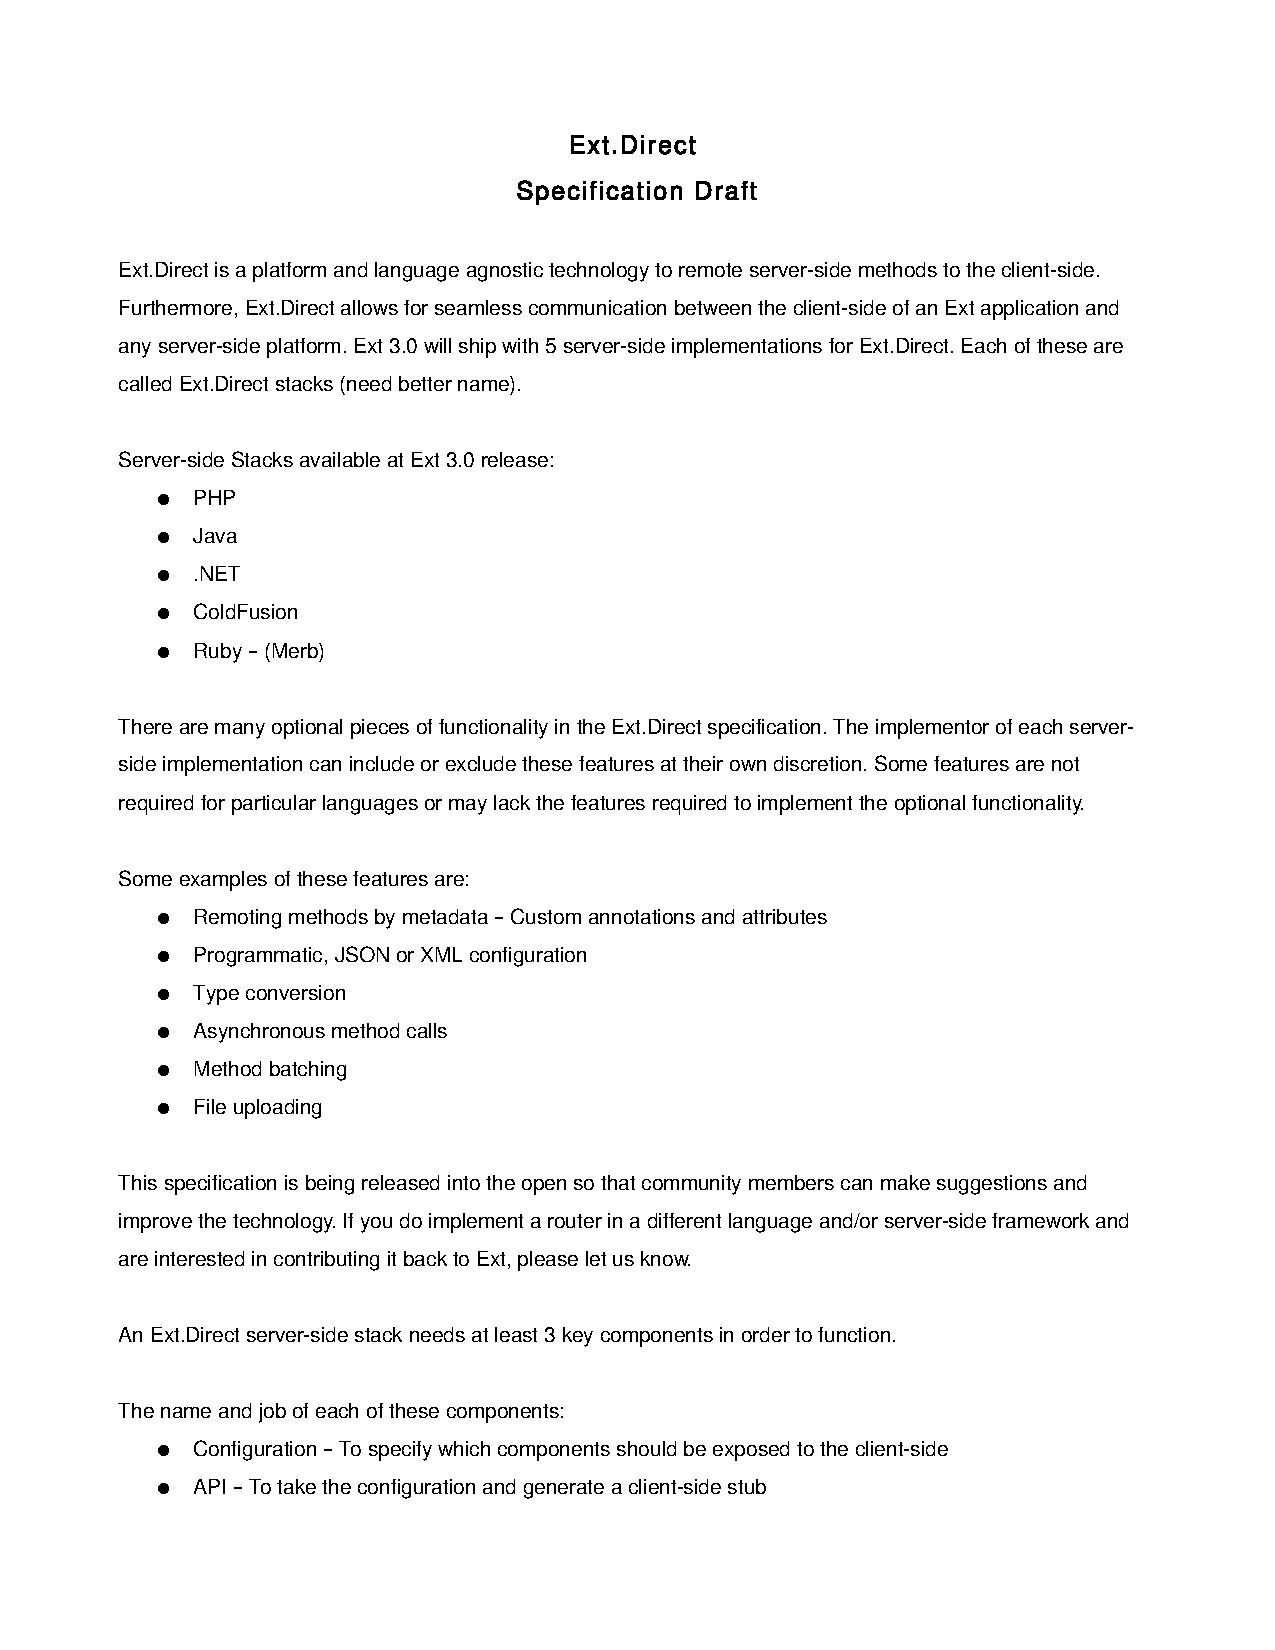
\includepdf{pdf/extdirect.pdf}

\section{Java Content Repository Spezifikation}
%
\includepdf{pdf/jcr-spec.pdf}

